\chapter{DCDT Calibration Procedure}

\section{Introduction}

Direct Current Displacement Transducers or Direct Current Differential Transformers (DCDTs) are devices
used to very precisely measure rectilinear motion. In the transducer there are a primary and two secondary
coils wound around a tube through which the core of the transducer travels. The primary coil is driven
with a high frequency alternating current waveform. The alternating magnetic field created is coupled into
the two counter wound secondary coils via a magnetically permeable core. The position of the core determines
how much coupling there is between the primary and each of the secondary coils. Therefore the output of the
secondary coils is a linear function of displacement. Which side of center the core is on in encoded by the
phase of the output with respect to the input. We use DCDTs which are excited by a direct current input and
provide a direct current output. The creation of the driving waveform and conditioning of the signal output
is all done on board the transducer.

In this appendix I will briefly show the calibration procedures used to calibrate our DCDTs in the laboratory.
Calibrations should be performed semi-annually. If a transducer's response has changed significantly, it
could be time to replace the transducer. Other problems such as response hysteresis and noise should
be noted as well.

\section{Calibration procedure}
Calibration of displacement transducers is accomplished with a NIST traceable transfer
calibration standard. Using the electronics that will be used during the experiment, the
transducer is placed a number of displacements using a vernier height gage. The response
is recorded and a calibration curve constructed. The calibration procedure is as follows:

\begin{enumerate}
\item Connect the DCDT to the appropriate electronics on the biax (i.e.
    vertical or horizontal axis). Allow a minimum of 10-15 minutes warm-up to
    ensure that the transducer will not drift. You will notice that the transducers
    and cores get very warm. It is best to have the transducer near its null position
    during warm-up.
    
\item Mount the transducer to a ring-stand using a universal clamp and adjust it to be perpendicular to
         the table.
         
\item Using a 4-40 all thread segment, mount the core of the transducer to the vernier height gage.

\item Set the height gage to an even millimeter increment.

\item  Make sure the transducer zero settings are close to their minimum values and that
          no DC offsets are being applied.
      
\item Plug the 4.5 digit multimeter into the appropriate bananna plugs on the
    biax front panel. 
        
\item Slide the transducer over the core and find the bottom of the output range. Lock it in place on the ring stand.
        
\item Take a reading at this zero displacement condition from the panel meter. Record this value.

\item Move the transducer in 1 mm or 0.5 mm steps, depending on its range. A minimum of 10 displacement values should
         be measured over the range of the transducer. At each step record the output voltage of the system.

\item Plot the voltage (in mV) and displacement (in mm). Fit a line. There should not
     be any appreciable non-linear or hysteresis behavior. If there is, consider
     recalibrating or troubleshooting the transducer.

\item Update DCDT calibration numbers in the calibration file, logsheets, and your notes.
\end{enumerate}


\section{Typical measured response}

As an example of a typical load cell response, a calibration of a TransTek DCDT shows a very linear trend with no hysteresis (Fig.\ref{ex_dcdt_fit}).

% Figure %
\begin{figure}
	\centering
		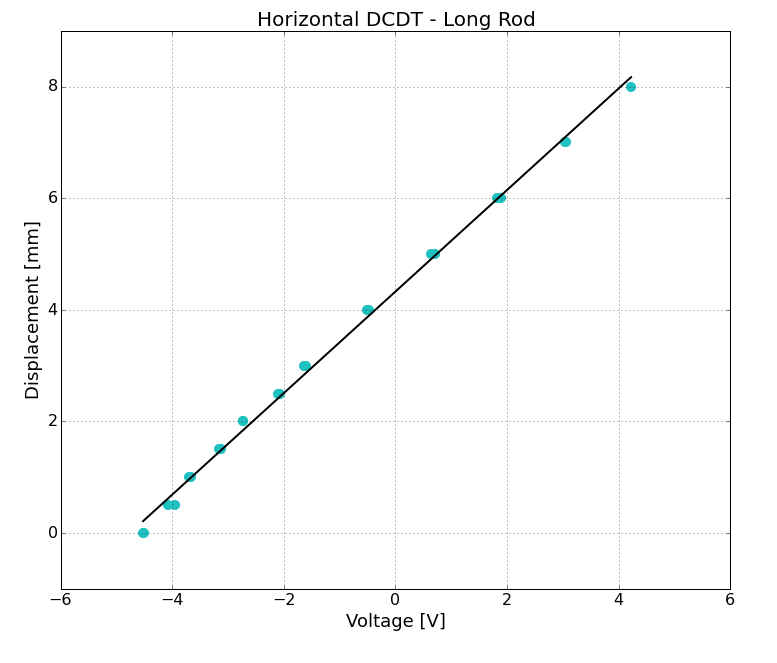
\includegraphics[scale=0.35]{appendix_dcdt_calibration/ex_dcdt_fit.png}
   	\caption{An example calibration obtained from a DCDT. }
  	\label{ex_dcdt_fit}
\end{figure}
% End Figure %
